\chapter{Model-based specification}
\label{chapter:specification}

In this chapter, we will look at \emph{model-based specification} --- one style of formal specification. We will look at the \emph{Alloy} language for specification, and how this can be used to model systems and check properties about the models. In the workshops, we will also look at a tool, called the \emph{Alloy Analyser} for bounded checking of Alloy specifications.

\section{What is formal specification?}

Formal specification is the use of mathematical notation to describe properties of a system. The use of mathematical notation provides precision that is not possible with natural language specification, which is subject to ambiguity and incompleteness. Formal specifications provide the specifier with a way to formally define \emph{what} a system must do, without saying \emph{how} it should do it. Thus, they are as formal as a programming language, but they do not constrain the design of the underlying algorithms or data structures.

Because formal specifications do not constrain design detail, and are independent of their implementation, they can be produced early in the project lifecycle; e.g.\ at the requirements and architectural design phases. At these phases, they are particularly valuable. As well as providing an unambiguous reference for system designers and implementers, the mathematical nature of formal specifications provides software engineers with the opportunity to \emph{prove} properties about the specification, such as correctness, completeness, and consistency, but also other properties, including safety and security.

In this chapter, we will use the \emph{Alloy} specification language \cite{jackson2012software}. Alloy is based on the Z language \cite{woodcock-using-z}, which is the most widely used and probably most widely known formal specification language. Alloy sacrifices the expressiveness of Z for computational tractability; that is, some expressive features in Z are removed to allow us to automatically check properties of Alloy specifications.

In this subject, we use Alloy for two reasons:

\begin{enumerate}
 \item It offers an intuitive notation.
 \item The Alloy Analyser tool for checking Alloy specifications is a state-of-the-art research prototype, which has been applied to many industry systems, and is supported by a large community of users.
\end{enumerate}


\section{What is model-based specification?}

Model-based specification is an approach to formal, system specification in which the system is defined as a state machine model. That is, there is a state representing the data in the system, and operations specify the transitions that can take the system from one state to another. This is much like the idea of a module/package in Ada: the variables define the state, and the subprograms define the transitions. The clean mapping from model-based specifications to modules is one reason that model-based specification has become the preferred method for formal specification, as opposed to axiomatic or algebraic approaches, which specify the properties of the systems via sets of axioms.

\paragraph{Model-based specification in the software engineering lifecycle.}
Model-based specification is not a requirements elicitation technique, nor is it generally a requirements engineering technique. Many model-based specifications are finalised during architectural design, once the components of the system are known. However, the formalisation of the behaviour of system components implicitly leads to a formalisation of those system requirements that the components are implement. As such, model-based specification falls over the phases of requirements engineering and architectural design. We should be comfortable with this, as in modern software engineering, the line between requirements and architectural design is blurred.

Figure~\ref{fig:specification:sdlc}, adopted from Sommerville \cite[Ch.\ 27]{sommerville10} shows the relationship between different activities in the early software engineering phases, and how model-based specification is typically carried out in parallel with other activities. Information flow between the activities is two-way --- information is always passed between the requirements and design phases.

\begin{figure}[!h]
\centering
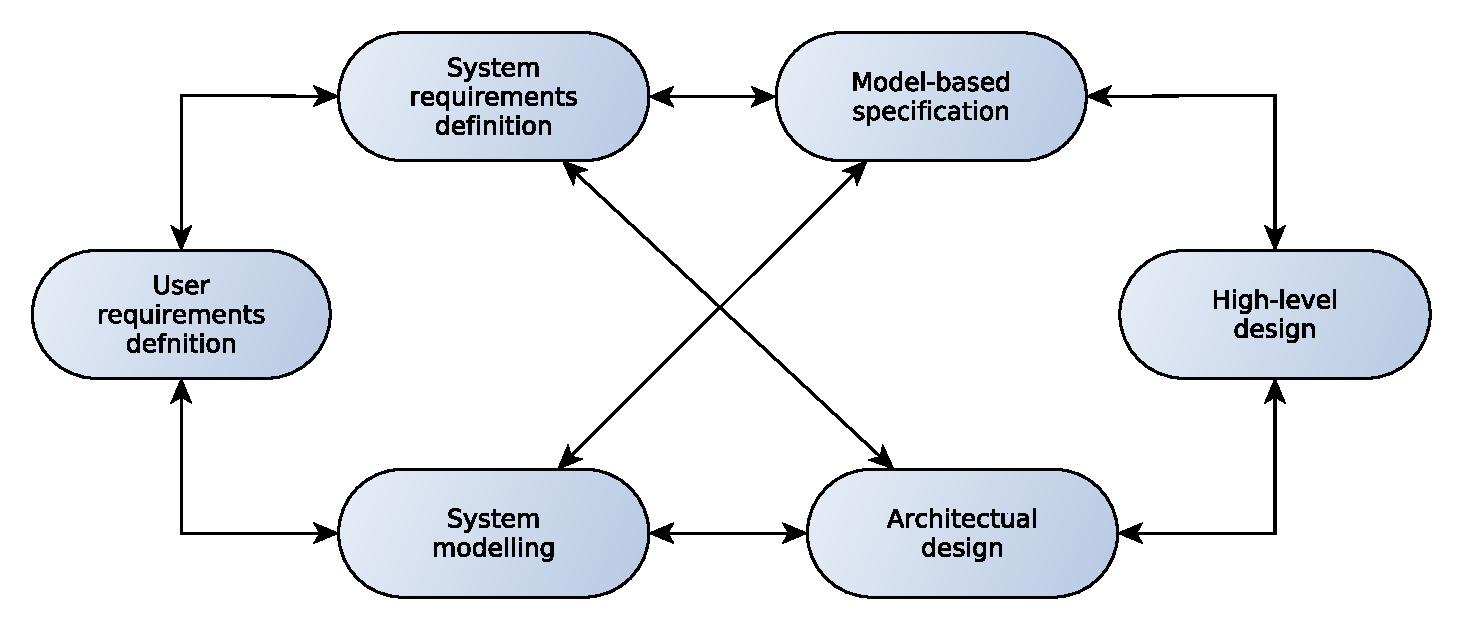
\includegraphics[scale=0.6]{\rootdir/specification/figures/specification-in-lifecycle}
\caption{Model-based specification in the software process.}
\label{fig:specification:sdlc}
\end{figure}

\paragraph{Languages for model-based specification.}
There are several well-known languages for model-based specification, including VDM, B, Z, and Alloy. These languages all have commonalities, especially that data types are based on sets and relations, and operations are specified using predicate logic. UML statecharts are another example of model-based specification, although the level of formality in these is less than in VDM, B, Z, and Alloy, as the intended areas of use are different.

\paragraph{Model-based specification and natural language.}
Like programming languages, formal, model-based specifications cannot be understood fully by a simple read over. As such, documenting the specification using natural language is important, just like commenting program code. Natural language descriptions not only allow the reader to understand the specification at a superficial level without having to worry about detail, but also allow the reader to understand the formal details, by guiding them through the meaning.


\section{The costs of formal specification}
\label{sec:specification:costs}

Using a rigorous process and method for formally specifying system properties can clearly be a costly exercise. The activity of specifying the precise detail of systems and sub-systems using mathematical notation requires careful thought and increased knowledge about the systems. Further, they must come under the same scrutiny of quality assurance using reviews and inspections as other requirements specification techniques. 

The question to be asked is: \emph{``Is the cost worth it?''}.

A major limitation to people using formal specification, even in high integrity domains, is that the perceived cost is too high. However, studies repeatedly show the following: the cost of specification is higher, but some of the added costs are recouped later in the process. Figure~\ref{fig:specification:costs-of-formal-specification}, taken from Phillips \cite{phillips89}, shows data from a project, comparing the number of errors found per thousand lines of code of using the Z specification language, against not using formal specification at all. The project from which the data comes from is the CICS project undertaken at IBM. The project introduced 268,000 lines of new code into a system already containing 500,000 lines of code. Of the new code, 48,000 lines was engineered from a formal specification written in Z, and Z was used at the product-, component-, and module-level design stages. Others studies show similar results.

\begin{figure}[!h]
\centering
\includegraphics[scale=0.6]{\rootdir/specification/figures/CICS-graph}
\caption{The costs of formal specification on the CICS project.}
\label{fig:specification:costs-of-formal-specification}
\end{figure}

Let's analyse this figure and ask ourselves why formal specification would \emph{reduce} the costs of later phases. There are a number of reasons for this:

\begin{enumerate}
 \item Using mathematical notation removes ambiguity from specifications, which is a cause of many problems in software. This helps to limit the amount of re-work in later phases, driving down their costs. In high-integrity systems, requirements typically change must less frequently than in say, enterprise systems, so the models do not require major changes every increment.

 \item Some cost incurred during design and implementation is simply trying to decide exactly what the behaviour of the system could be. Using natural language to specify requirements means that we can be shorthanded and therefore miss or ignore important detail. Using mathematical notation does not afford this because it is easy to show incompleteness, and many of the issues that generally present themselves during design and implementation must be solved during specification instead. In other words, the people doing the specification do some of the work typically undertaken at the design and implementation phases.


 \item Despite opinion to the contrary, designing and implementing a system from a formal specification is \emph{more} straightforward than doing so from natural language requirements. For a novice, this may not be the case, but for someone who is as comfortable with mathematical notation as they are with programming languages, this is most definitely the case.

 \item Using formal notation offers the possibility of \emph{proving} that our specification satisfied certain properties. Discovering in later phases that our specification does not satisfy some properties is more costly than discovering these in early phases.

 \item Post-release costs are reduced due to the fact that less mistakes are introduced over the process; or more accurately, the same number of mistakes are made, but more are made \emph{and found} during specification, rather than post release.
\end{enumerate}

A simple (and common) objection to formal specification is that it is just too hard: the formality is too difficult for the average programmer to grasp. I agree that this is case. I would not advocate employing formal specification on a project with programmers who have no experience at it. However, I disagree that this \emph{has to be} the case. The average programmer is already intelligent enough to have learnt a formal language: all programming languages are formal. As such, we know they are equipped to deal with formal languages, even at the specification language. 

However, an important extension to this argument is the following: \emph{formal specification is much simpler than programming --- we only have to specify \emph{what} a system should do, whereas our program must specify \emph{how} to do it}.

If programmers were trained in formal specification languages the same way they were trained in programming languages, reading and using formal specifications would not be an issue. Thus, the cost of formal specification would be \emph{significantly} less than the cost of implementation -- although its \emph{value} may not be.

That is not to say that formal specification should be used in every organisation or on every project: it is only cost effective when the cost of releasing software with faults is greater than the cost of preventing them. In environments where the biggest issue is responding to change (e.g.\ change of customer preferences, change of requirements from a client), ensuring the software is correct is not as high of a priority as getting something out that works for most normal cases.

In high integrity systems, formal specification is generally only applied to those parts of the system that contain high-integrity requirements. Other parts of the system, for example, data storage or user interface, are engineered using more standard techniques.

\section{Logic and set theory}

Most formal model-based specification languages are based on \emph{first-order predicate logic} and \emph{set theory}; both topics with which all students in this subject are expected to be familiar. 
The set theory part of Alloy contains the standard set theoretic concepts, such as set comprehension, power sets, set operators (union, intersection, subset, etc.), Cartesian products, relations, and functions. The predicate logic part of Alloy contains propositional operators (``and'', ``or'', ``implies'', etc.) and existential and universal quantifiers (``for all'', ``there exists'').

The most important concepts with which you are expected to be familiar are:

\begin{itemize}

 \item First-order logic: conjunction (``and''), disjunction (``or''), implication, negation, universal quantification (``for all''), and existential quantification (``there exists'').

 \item Set theory: set membership, set comprehension, set union, set intersection, set difference, and subsets.

 \item Relations: Cartesian product, domain and range of relations, sequences, partial functions, and total functions.

\end{itemize}

If you are not familiar these concepts, or the details are hazy, Chapter 3 of Daniel Jackson's book \emph{Software Abstractions: Logic, Language, and Analysis} \cite{jackson2012software}, provides a detail description of these concepts, and how to express them in Alloy.

If you cannot access this, Chapters 2-9 in Woodcock and Davies book ``Using Z'' \cite{woodcock-using-z} provides a detailed description of basic logic and set theory, which can also be read lightly to pick up the most important aspects. A PDF version of this book is available on the LMS for download.

\subsubsection{Why sets and predicates?}

Most model-based languages are based on sets and predicates. The reasons are quite simple: 

\begin{enumerate}

 \item Set theory (sets, relations, functions, etc.) provides us with enough notation to specify the data of any system. Just as importantly though, it \emph{restricts} us from specifying design detail, and forces us to think more abstractly --- something which is important at the specification level. 

 \item Predicate logic provides us with sufficient expressive power to specify what changes the data of a system can undergo over time (or the effect of operations on data). Just as importantly, it \emph{restricts} us from specifying \emph{how} those changes should be implemented.

These first two points are important: requirements engineering is already difficult enough without us thinking about design and implementation problems at the same time.

 \item Together, proof theory and understanding of set theory and predicate logic is strong enough that we can prove many properties specified using these parts. We can take advantage of hundreds of years of work in these areas and apply this to software engineering --- a field that is relatively new in comparison.

\end{enumerate}


\begin{example}
As an example of using logic and set theory to specify software and system behaviour, and how this differs from programming, consider the trivial example of sorting a list of integers.

To specify the behaviour of a procedure that takes a (possibly unsorted) list and sorts it, we have to say that:

\begin{enumerate}

 \item each element in the input list is present in the output list (that is, the output list is a permutation of the input list); and

 \item each element of the output list is less than or equal to the next (that is, the list is sorted).

\end{enumerate}


We can specify what it means for a list of integers to be sorted:
\[
 \forall list : \seq \integer @ ~~sorted(list)~~ \iff~~  \forall i : 1 \upto \#list - 1 @ list(i) \leq list(i + 1)
\]
This states that, for all sequences of integers, that sequence is sorted \emph{if and only if}: for each index (except the last) in the list, the integer at that index is less than or equal to the integer at the next index.

We can also specify what it means for one list to be a permutation of the other.
\[
 \forall a, b : \seq \integer @  ~~permutation(a,b)~~ \iff~~  \forall el : \integer @ count(el, a)  = count(el, b)
\]
 
in which $\mathit{count}$ is defined as:
\[
 \forall el : \integer; list : \seq \integer; c : \nat @~~ count(el, list) = c ~~\iff~~
    c = \#(list\rres \{el\})
\]

That is $count(el, list) = c$ if and only if $c$ is the number of elements when we take the \emph{range restriction} of $list$ on $el$ only.

Finally, we can specify the precondition and postcondition of a procedure using these concepts:

\textbf{procedure}  $sort (in\_list : \textbf{in} \seq \integer; out\_list : \textbf{out} \seq\integer)$ \textbf{is}

\vspace{-2mm}

\quad \textbf{pre} ~$\#in\_list > 1$

\vspace{-2mm}

\quad \textbf{post} $sorted(out\_list) \land is permutation(in\_list, out\_list)$

Here, we have added a superficial precondition that the list is not empty.

So, this example specifies the functional behaviour of sorting a list, but does NOT specify \emph{how} the list should be sorted. Any correct algorithm for sorting integers will suffice to fulfil the specification above.

\end{example}

\begin{example}
Using the definitions above, we can specify the behaviour of a binary search algorithm in a straightforward manner:

\textbf{procedure}  $binary\_search (list : \textbf{in} \seq \integer; target : \textbf{in}\ \integer; index : \textbf{out}\ \integer)$ \textbf{is}

\vspace{-2mm}

\quad \textbf{pre} ~$sorted(list)$

\vspace{-2mm}

\quad \textbf{post} $target = list(index) \lor (target = -1 \iff target \notin \ran(list))$

In this example, we have called the procedure ``$binary\_search$'', but only because we specify in the precondition that the input list must be sorted. Other than this, the algorithm is not constrained by any particular binary search algorithm (e.g.\ recursive or iterative), and in fact, does not truly constrain it to a binary search algorithm at all.

We can see from this example: specifying binary search behaviour is much neater than specifying the algorithm to achieve it.

\end{example}

\section{Introduction to Alloy}

In this chapter, we will present the Alloy language. We will present only a small subset of the language, but it is enough to allow specification of and reasoning about  abstract state machines. The Alloy has a rich notation for combining predicates, which allow flexible and incremental building of specifications. We will not go into detail on all of these operators, but we will use some of the basic components to enable clean specification.

An Alloy reference manual is available online at:

 \url{http://alloy.mit.edu/alloy/documentation/book-chapters/alloy-language-reference.pdf}

It provides detailed syntax and semantic definitions. 


\subsection{Key characteristics}

There are a few key ideas to Alloy that are worth noting.

\subsubsection{Alloy = logic + language + analysis}

The complete Alloy framework consists of three parts:

\begin{enumerate}
 \item \emph{Logic}: This consists of first-order predicate logic, plus a simple relational calculus.
 \item \emph{Language}: This consists of a handful of operators for structuring specifications, such as specifying types, predicates, functions, and assertions.
 \item \emph{Analysis}: This performs an exhaustive search (in bounded domains) for counterexamples using SAT (satisifiability check).
\end{enumerate}


\subsubsection*{Non-specialised logic}

The logic of Alloy is not tied to a particular paradigm, such as concurrent modelling or state machines. One can write models of this type in Alloy, and indeed, in this subject, we will focus primarily on using Alloy as a model-based language for specifying state machines.

\subsubsection*{Not proof, but counterexamples}

The focus of the Alloy Analyser is not to \emph{prove} a model has a particular property, but instead is to find counterexamples that demonstrate the property does not hold. Finding such a counterexample demonstrates that the property does not hold, while failing to find one demonstrates that the property \emph{may} hold.

In particular, Alloy encourages the use of small, finite domains on which to do analysis. That is, rather than search for a counterexample in a large or finite set of objects, it encourages (at least during initial analysis) to use small domains of only a few objects; e.g.\ only three usernames, URLs, and passwords. This approach has two advantages:

\begin{enumerate}
 \item Using small domains means the analysis is much faster, as there are less objects to check.
 \item Most assertions are (initially) wrong, and small counterexamples to them can be found. Having small counterexamples means understanding the counterexample itself is more straightforward.
\end{enumerate}

The aim of the Alloy Analyser though is not to search a handful of arbitrary ``test'' cases in a small domain, but search for \emph{all} possible cases in that domain. The real domain may be infinite, but a small, finite set representing that domain will find \emph{almost} all flaws.

\section{Alloy Logic}

In this section, we present the logic used in Alloy, which is based on predicate logic and relational calculus.

We will use the example of a password management system, such as \emph{LastPass}, which remembers the username and password combinations for particular websites (represented by their URL).

\subsection{Everything is a relation}

Alloy uses relations for all data types, including scalars and sets. Sets are just unary relations; e.g.:

\begin{alloy}
 Username = {(U0), (U1), (U2)}
 URL = {(UR0), (UR1), (UR2)}
 Password = {(P0), (P1), (P2)}
\end{alloy}

scalars are just singleton sets:

\begin{alloy}
 myUsername = {(U0)}
 myPassword = {(P1)}
\end{alloy}

and relations are just sets of tuples:

\begin{alloy}
 passwords = {(U0, P1), (U1, P2)}
\end{alloy}

This above represents a mapping of usernames to passwords, in which username \texttt{U0} maps to password \texttt{P1}. An alternative could be to have a password for a particular URL:

\begin{alloy}
 urlPasswords = {(U0, UR0, P1), (U0, UR1, P2), (U1, UR0, P2)}
\end{alloy}

Here, user \texttt{U0} has two passwords for two different URLs (\texttt{UR0} and \texttt{UR1}), while user \texttt{U1} has only one password.

An important restriction of relations in Alloy is that \emph{all relations are first-order}; that is, we cannot have sets of sets, or relations of relations. If using a set of sets is a natural way to represent a problem, we instead need to find another representation. This restrictions are is what permits the Alloy language to be (relatively) easily analysed by automated tools.


\subsection{Operators}

\paragraph{Set operators}
Sets (represented as unary relations) are a commonly-used data type in formal modelling. In Alloy, the main set operators are included in the logic:
%
\begin{center}
\begin{tabular}{lll}
\toprule
 Operator & Meaning & Example\\
\midrule
 \texttt{+}  & union         & \texttt{\{(U0)\} + \{(U1)\}}\\
 \texttt{\&} & intersection  & \texttt{\{(U0)\} \& \{(U1)\}}\\
 \texttt{-}  & difference    & \texttt{\{(U0), (U1)\} - \{(U1)\}}\\
 \textbf{in} & subset        & \texttt{\{(U1)\} \A+in+ \{(U0), (U1)\}}\\
 \texttt{=}  & equality      & \texttt{\{(U0), (U1)\} = \{(U0), (U1)\}}\\
\bottomrule
\end{tabular}
\end{center}

\paragraph{Cross product}
A cross product, represented using the operator $\times$ in set theory, is represented as the following in Alloy:
%
\begin{center}
\begin{tabular}{lll}
\toprule
 Operator & Meaning & Example\\
\midrule
 \texttt{->}  & cross product & \texttt{Username->Password}\\
\bottomrule
\end{tabular}
\end{center}

As an example, consider the cross products taken from URLs, usernames, and passwords:

\begin{alloy}
 Username = {(U0, U1, U2)}
 URL = {(UR0, UR1, UR2)}
 Password = {(P0, P1, P2)}
 Username->Password = {(U0, P0), (U0, P1), (U0, P2),
                       (U1, P0), (U1, P1), (U1, P2),
                       (U2, P0), (U2, P1), (U2, P2)}
 Username->URL->Password = {(U0, UR0, P0), (U0, UR0, P1), (U0, UR0, P2),
                            (U0, UR1, P0), (U0, UR1, P1), (U0, UR1, P2),
                            ...
                            (U2, UR2, P0), (U2, UR2, P1), (U2, UR2, P2)}
\end{alloy}

\paragraph{Join operators}
There are two operators for joining relations in Alloy: 
%
\begin{center}
\begin{tabular}{lll}
\toprule
 Operator & Meaning & Example\\
\midrule
 \texttt{.}  & dot join & \texttt{URL.passwords}\\
 \texttt{[]} & box join & \texttt{(Username->Password)[myUsername]}\\
\bottomrule
\end{tabular}
\end{center}

These operators are are related via the following properties:

\begin{alloy}
  a.b = b[a]
  a.b.c[d] = d.(a.b.c)
\end{alloy}

A dot join is a relational join, which maps the range of the relation on the left to the domain of the relation on the right. For example:

\centerline{
  \xymatrix@R-1.5pc@C=5em{
    \texttt{A}                      & \texttt{B}               & \texttt{A.B}\\
    \texttt{(a,b)}\ar[rd]\ar[rddd]  & \texttt{(a,d,c)}         & \texttt{(a,c,c)} \\
    \texttt{(a,c)}\ar[rd]           & \texttt{(b,c,c)}\ar[ur]  & \texttt{(a,a,d)}\\
    \texttt{(b,d)}                  & \texttt{(c,c,c)}\ar[ur]  & \\
                                    & \texttt{(b,a,d)}\ar[uur] & \\
   }
}

For the relations:

\begin{alloy}
  myUsername = {(U0)}
  myUrl = {(UR1)}
  urlPasswords = {(U0, UR0, P1), (U0, UR1, P2), (U1, UR0, P2)}
\end{alloy}

the following hold:

\begin{alloy}
  myUsername.urlPasswords = {(UR0, P1), (UR1, P2)}
  myUsername.urlPasswords[myUrl] = {(P2)}
\end{alloy}

which matches the \texttt{U0} in \texttt{myUsername} to the same value in \texttt{urlPasswords}. 

\paragraph{Restriction and override}
The concepts of domain restriction, range restriction, and function override are represented as follows:
%
\begin{center}
\begin{tabular}{lll}
\toprule
 Operator & Meaning & Example\\
\midrule
 \texttt{<:} & domain restriction & \texttt{urlPasswords <: myUrl}\\
 \texttt{:>} & range restriction  & \texttt{urlPasswords :> Password}\\
 \texttt{++} & function override  & \texttt{urlPasswords ++ (myUsername->myUrl->newPassword)}\\
\bottomrule
\end{tabular}
\end{center}

Function override is defined as: \A|A ++ B|~~ = ~~\A|(A - (domain[B] <: A) + B)|.

Informally, domain restriction, \A|A <: B| takes the relation \texttt{A} and restricts it to contain only the tuples whose domain is in \texttt{B}, while range restriction, \A|A :> C| restricts \texttt{A} to contain only the tuples whose range is in \texttt{C}. For example, if we have:

\begin{alloy}
  myUsername = {(U0)}
  myUrl = {(UR1)}
  someUsernames = {(U0), (U1)}
  somePasswords = {(P1), (P3)}
  newPassword = {(P4)}
  urlPasswords = {(U0, UR0, P1), (U0, UR1, P2), (U1, UR0, P2), (U2, UR3, P3)}
\end{alloy}

then the following hold:

\begin{alloy}
  urlPasswords <: someUsernames = {(U0, UR0, P1), (U0, UR1, P2), (U1, UR0, P2)}
  urlPasswords :> somePasswords = {(U0, UR0, P1), (U2, UR3, P3)}
\end{alloy}

For override, we supply at least one new tuple, which is added to the relation, but with the further constraint that it \emph{overrides} the value of any existing tuple with the same domain; e;g.:

\begin{alloy}
  urlPasswords ++ (myUserName->myUrl->newPassword) = 
      {(U0, UR0, P1), (U0, UR1, P4), (U1, UR0, P2), (U2, UR3, P3)}
\end{alloy}

\paragraph{Propositional logic operators}

\begin{center}
\begin{tabular}{lll}
\toprule
          & Alternative &         \\
 Operator & Operator    & Meaning \\
\midrule
 \texttt{!}  &  \texttt{\textbf{not}}  & negation\\
 \texttt{\&\&} &  \texttt{\textbf{and}}  & conjunction\\
 \texttt{||} &  \texttt{\textbf{or}}  & disjunction\\
 \texttt{=>} &  \texttt{\textbf{implies}}  & implication\\
 \texttt{<=>} &  \texttt{\textbf{iff}}  & if-and-only-if\\
\bottomrule
\end{tabular}
\end{center}

\paragraph{Predicate logic quantifiers}
Assuming that \texttt{x} is a variable, \texttt{e} is a set expression, and \texttt{F} is a formula, the following are valid formula:

\begin{center}
\begin{tabular}{lll}
\toprule
 Operator & Meaning\\
\midrule
  \A+all x : e | F+  & \texttt{F} holds for every \texttt{x} in \texttt{e}\\
  \A+no x : e | F+  & \texttt{F} holds for no \texttt{x} in \texttt{e}\\
  \A+some x : e | F+  & \texttt{F} holds for at least one \texttt{x} in \texttt{e}\\
  \A+lone x : e | F+  & \texttt{F} holds for at most one \texttt{x} in \texttt{e}\\
  \A+one x : e | F+  & \texttt{F} holds for exactly one \texttt{x} in \texttt{e}\\
\bottomrule
\end{tabular}
\end{center}

For example, the following two predicates specify that: (1) there is at least one password for the user corresponding to \texttt{myUsername}; and (2) no username has more than one password:

\begin{alloy}
(1) some pwd : Password | (myUsername->pwd) in passwords
(2) all user : Username | lone pwd : Password | pwd in user.passwords
\end{alloy}

The last four of these keywords can also be applied to \emph{relations}:

\begin{center}
\begin{tabular}{lll}
\toprule
 Operator & Meaning\\
\midrule
 \A+no e+  & \texttt{e} has no elements/tuples\\
 \A+some e+  & \texttt{e} has at least one element/tuple\\
 \A+lone e+  & \texttt{e} has at most one element/tuple\\
 \A+one e+  & \texttt{e} has exactly one element/tuple\\
\bottomrule
\end{tabular}
\end{center}

For example, we can re-write the two examples above as:

\begin{alloy}
(1) some myUserame.passwords
(2) all user : Username | lone user.passwords
\end{alloy}

\paragraph{Set declarations}
In predicates and other constructs that use sets, modifiers are used to restrict the elements in declarations:

\begin{center}
\begin{tabular}{lll}
\toprule
          &         \\
 Operator & Meaning \\
\midrule
 \A+x : set e+ & \texttt{x} is a subset of \texttt{e}\\
 \A+x : one e+ & \texttt{x} is a singleton subset of \texttt{e}\\ 
 \A+x : lone e+ & \texttt{x} is an empty or singleton subset of \texttt{e}\\ 
 \A+x : some e+ & \texttt{x} is a non-empty subset of \texttt{e}\\ 
 \A+x : e+      & \A+x : one e+\\
\bottomrule
\end{tabular}
\end{center}

\paragraph{Set comprehensions}
New sets can be constructed from expressions:

\begin{center}
\begin{tabular}{lll}
\toprule
          &         \\
 Operator & Meaning \\
\midrule
 \A+{x : e, y : f | F}+ & A set of tuples that satisfy formula \texttt{F}\\
\bottomrule
\end{tabular}
\end{center}

We can construct a set of usernames that have the password \texttt{myPassword}:

\begin{alloy}
  {user : Username | user in password.myPassword}
\end{alloy}

\paragraph{Cardinalities}

\begin{center}
\begin{tabular}{lll}
\toprule
          &         \\
 Operator & Meaning \\
\midrule
 \A+#e+ & The number of tuples in expression \texttt{e}\\
 \A+0,1,2+ & Integer literals\\
 \A|+|, \A|-|  & Addition, subtraction\\
 \A|=|, \A|<=|, \A|<|, \A|>=|, \A|>|  & Arithmetic operators\\
\bottomrule
\end{tabular}
\end{center}

\textbf{Note} that there is no multiplication or division! Multiplication and division are not included in the language because SAT solvers are typically unable to deal with them in the general case.

\paragraph{\texttt{let} formula and expressions}
A \texttt{\textbf{let}} expression is a shorthand:

\begin{center}
\begin{tabular}{lll}
\toprule
          &         \\
 Operator & Meaning \\
\midrule
 \A+let x = e | formula+\\
 \A+let x = e | expression+\\
\bottomrule
\end{tabular}
\end{center}

For example:

\begin{alloy}
all user : Username | let p = user.passwords | lone p && some p
\end{alloy}

\section{Alloy Language}

The Alloy language provides constructs to structuring specifications using the logic presented in the previous section.


\subsection{Modules}

Alloy modules are analogous to modules in programming languages, so are used to model self-contained specifications that can be imported into other modules and re-used.

\subsection{Signatures}
 
Signatures are essentially type declarations:

\begin{center}
\begin{tabular}{ll}
\toprule
 Operator & Meaning\\
\midrule
 \A+sig A {}+ & Declare a set of atoms called \texttt{A}\\
 \A+sig B {}+ & Declare a set of atoms called \texttt{B}, which is disjoint from \texttt{A}\\[3mm]
 \A+sig A, B {}+ & As above\\[3mm]
 \A+sig B extends A {}+ & Declate sets \texttt{A} and \texttt{B} where \texttt{B} a subset of \texttt{A} (\texttt{B in A})\\[3mm]
 \A+abstract sig A {}+ & An \emph{abstract} set of atoms\\
 \A+sig B, C extends A {}+ & B and C are disjoint, and (\texttt{A=B+C})\\[3mm]
 \A+sig A {f : e}+ & \texttt{f} is a binary relation of type \A|f : A -> one e| \\
\bottomrule
\end{tabular}
\end{center}



For example, we can construct types for keeping track of passwords at particular URLs:

\alloyfile{linerange={16-19}}{\rootdir/specification/code/lastpass.als}

Here, \texttt{PassBook} models a set of ``known'' username and URL combinations, and the passwords for these. There is, at most, one password per pair (\A+passwords+ is a function).

\subsection{Facts}

Facts are (possibly named) constraints that are always assumed to hold. They are introduced in two different ways:



\begin{center}
\begin{tabular}{ll}
\toprule
 Operator & Meaning\\
\midrule
 \A+fact f { F }+ & Declare a fact called \texttt{f} that introduces a formula \texttt{F}.\\
 \A+sig A { ... } { F }+ & Declare a signature \texttt{A} with formula \texttt{F}\\
\bottomrule
\end{tabular}
\end{center}

For example, we can express that a \texttt{PassBook} can have at most one password for each user/URL pair:

\alloyfile{linerange={21-24}}{\rootdir/specification/code/lastpass.als}

We could also have introduced this explicitly in the signature:

\begin{alloy}
sig PassBook {known : Username -> URL, password : known -> one Password}
             { all user : Username, url : URL | lone password[user][url]}
\end{alloy}

In this example, we need not quantify \A{pb : PassBoook} in the \A+all+, because the variables declared in the signature are accessible.

Such facts can be used to model \emph{invariants} over the data types: constraints that always hold for the data types.

\subsection{Predicates}

Predicates are named formula with declared parameters. Predicates can be accessed from within other predicates.

\begin{center}
\begin{tabular}{ll}
\toprule
 Operator & Meaning\\
\midrule
 \A+pred p [x : e] { F }+ & Declare a predicate called \texttt{p}, which has variable(s) \texttt{x}, and formula \texttt{F}\\
\bottomrule
\end{tabular}
\end{center}

In this subject, we will primarily be using predicates to introduce \emph{operations} over a state. That is, a set of signatures will define the state space, and predicates will define the possible transitions over that state space.

For example, we can have operations that add and delete passwords to a PassBook:

\alloyfile{linerange={26-36}}{\rootdir/specification/code/lastpass.als}

Note the naming convention used in this predicate as it is used to define an operation. There are \emph{two} variables of type \texttt{PassBook}:
(1) \A+pb+, which refers to the value of the variable \emph{before} the operation is ``executed'' (called the \emph{pre-state} value); and (2) \A+pb'+, which refers to the value \emph{after} the operation has executed (called the \emph{post-state} value). The post-state variable is distinguished from the pre-state variable using a single quote mark (e.g.\ \A{pb'}).

The \texttt{add} predicate specifies an operation with a pre-state variable \texttt{pb}, post-state variable \texttt{pb'}, and three input variables \texttt{user}, \texttt{url}, and \texttt{password}. 

The first line of the predicate part states that there is not already a password for this user/URL pair (the set formed by \texttt{pb.password[user][url]} is empty). This is a \emph{precondition}: the behaviour of the operation is not defined if this holds.

The second line is the \emph{postcondition}, which specifies what transition should happen if the precondition holds. In this case, an override (\texttt{++}) is used to specify that the post-state value, \texttt{pb'}, is the same as the pre-state value \texttt{pb}, but with the new details added.

The \texttt{delete} predicate specifies an operation that deletes a password from the PassBook. The precondition requires that a password exists, and the postcondition uses set difference to remove the tuple from the relation of passwords.

Predicates can be accessed within other predicates. For example, we could break the precondition of the \A+add+ predicate into its own predicate, and reference this:

\begin{alloy}
//True if and only if the user has no password for this URL
pred preAdd [pb : PassBook, url : URL, user: Username] {
    no pb.password[user][url] 
}

//Add a password for a new user/URL pair
pred add [pb, pb': PassBook, url : URL, user: Username, pwd: Password] {
    preAdd [pb, url, user]
    pb'.password = pb.password + (user->url->pwd)
}
\end{alloy}

The semantics of the \A+add+ operation is exactly as if the body of \A+preAdd+ was included where it was referenced, with the appropriate variable renamings. 

\textbf{Note} that this is not sequence composition. That is, \A+preAdd+ is not ``executed'', followed by the line after it. The formulae in \A+preAdd+ and \A+add+ are evaluated as one larger conjunction.

\subsection{Functions}

Functions are named expressions with declared parameters and expressions. They can be `invoked' by predicates or other functions by providing an expression for each parameter.

\begin{center}
\begin{tabular}{lp{9cm}}
\toprule
 Operator & Meaning\\
\midrule
 \A+fun f [x : e1] : e2 { F }+ & Declare a function called \texttt{f}, which has variable(s) \texttt{x}, formula \texttt{F}, and is of type \texttt{e2}\\
\bottomrule
\end{tabular}
\end{center}

For example, we can lookup the password for a given user/URL pair:

\alloyfile{linerange={44-47}}{\rootdir/specification/code/lastpass.als}

Note the expression/type given to the function: (\A{lone Password}). This function can be used as an expression as part of another formula. For example:

\alloyfile{linerange={49-52}}{\rootdir/specification/code/lastpass.als}

\subsection{Assertions}

Assertions are named constraints that are intended to follow from a model. We can express assertions using formula using:

\begin{center}
\begin{tabular}{ll}
\toprule
 Operator & Meaning\\
\midrule
 \A+assert a { F }+ & Declare an assertion called \texttt{a}, with the formula \texttt{F}\\
\bottomrule
\end{tabular}
\end{center}

For example, we can express the following assertion which says that the \texttt{add} predicate ``works'':
\alloyfile{linerange={64-68}}{\rootdir/specification/code/lastpass.als}

Assertions can be checked by the Alloy Analyser (see Section~\ref{sec:specification:alloy-analyser}).

Typically, assertions play two roles: (1) to express some properties that we should hold on the model, which we can then check to see if there are flaws in our model (or flaws in our assertions!); and (2) to express essential properties of the model that are higher than facts or properties; e.g.\ relationship between predicates; which give us a better understanding of the model itself, and possible ways to refine or restructure it.

\subsection{The complete \A+LastPass+ example}

\alloyfile{}{\rootdir/specification/code/lastpass.als}

\section{Analysis with the Alloy Analyser}
\label{sec:specification:alloy-analyser}

The Alloy language supports two types of construct that are related specifically to the Alloy Analyser. That is, they say nothing about the model itself, but are merely there to tell the analyser what to check, and to provide some parameters for this checking.

In these notes, we briefly discuss the main concepts in analysing Alloy models, and we will explore this more in the workshops.


\subsection{Runs}

The \A+run+ command instructs the analyser to search for instances of values that satisfy a predicate:
\begin{center}
\begin{tabular}{lp{12.5cm}}
\toprule
 Operator & Meaning\\
\midrule
 \A+run p scope+ & Find a valid binding of variables for predicate or function \A+p+, such that these values satisfy \A+F+, using the declared scope.\\
\bottomrule
\end{tabular}
\end{center}

For example, given the operation \A+add+ defined in the previous section, we can check that the \A+add+ is \emph{satisfiable} in a domain of size three using:

\begin{alloy}
run add for 3
\end{alloy}

This instructs the analyser to search for values for the variables, assuming that there are three instances of each signature in the universe; that is, three usernames, three URLs, three passwords, and three passbooks. We can restrict different variables to have different sizes:

\begin{alloy}
run add for 3 but 2 PassBook
\end{alloy}

This specifies that the domain should be of size three, except only two pass books.

If an instance can be found, this means that the predicate/function is indeed satisfiable. If an instance \emph{cannot} be found, this means predicate/function is \emph{possibly} unsatisfiable. It may be that the scope we used is simply not large enough to find a combination that satisfies the formula.

The idea of scope is discussed in more detail in Section~\ref{sec:specification:analyser:scope}.

\subsection{Checks}

The \A+check+ command instructs the analyser to search for instances of values that \emph{violate} an assertion --- a \emph{counterexample} to the assertion:
\begin{center}
\begin{tabular}{lp{12.5cm}}
\toprule
 Operator & Meaning\\
\midrule
 \A+check a scope+ & Find a counterexample to the assertion \A+a+, such that these values satisfy \A+not F+, using the declared scope.\\
\bottomrule
\end{tabular}
\end{center}

For example, given the assertion \A+addWorks+ defined in the previous section, we can attempt to find a counterexample to the assertion in a domain of size three using:

\begin{alloy}
check addWorks for 3
\end{alloy}

If a counterexample can be found, this means that the assertion does not hold on the model; i.e.\ the assertion is incorrect. If a counterexample cannot be found, then the assertion \emph{may} hold, or there may be a counterexample that exists outside of the specified scope.

\subsection{Scope}
\label{sec:specification:analyser:scope}

 The idea of scope is straightforward. The Alloy Analyser does \emph{bounded} checking, meaning that it can (potentially) try every combination of assignments of instances to variables -- although the searching algorithms are much more sophisticated and eliminated many infeasible combinations early on.

The scope can be modified to increase or decrease the number of instances that are used in the search. For example, we can use the following:

\begin{alloy}
run add
run add for 5
run add for 5 but 3 PassBook
run add for 5 URL, 5 Username, 10 Password, 2 PassBook
\end{alloy}

The first line omits a scope, in which case the default scope of three is used. The second command specifies that five instances of all signatures should be used, while the third says the same, except only create three signatures for \A+PassBook+. The final one explicitly lists the number of instances for each signature type.

There are several other ways to restrict the scope used in analysis. See Jackson's book on Alloy \cite{jackson2012software} for information on these.

\subsubsection{The small scope hypothesis}

By finding instances and counterexamples to predicates, functions, and assertions, we are essentially just doing exhaustive testing using a bounded set of instances. As such, we cannot \emph{prove} that an assertion holds for all instances in the universe. This is essentially \emph{like} testing, but in actually, it is much more powerful. 

The Alloy philosophy relies on the \emph{small scope hypothesis}, which is:

\begin{quote}
 \emph{Most faults have small counterexamples}.
\end{quote}

That is, if an assertion in incorrect, it \emph{often, but not always}, has a counterexample that exists in a small scope of around 3-5 instances per signature. The Alloy Analyser exhaustively analyses all cases within the declared scope, therefore, if a counterexample exists within that scope, it will be found. This is in contrast to testing, which will select a small subset of the scope as test inputs. 

Using larger scopes increases the chance of finding a counterexample of course, but also takes more CPU time and memory to analyse. A good strategy is to start with a small scope of three, which is usually sufficient to find flaws in our models early on, eliminate these flaws, and once all of our runs and checks pass, extend the scope to be much larger, and leave the analyser to search for a period while we go for a coffee.


\section{Abstraction and incremental specification of state machines using Alloy operators}

In the previous section, we saw how to create operation predicates from smaller operation predicates; e.g.\ by specifying the precondition of the \A+add+ operation in its own predicate \A+preAdd+ and referencing this. Using predicates as building blocks in this way is an excellent abstraction mechanism that can be used to our advantage in specifying systems.

The formal specification process is not as simple as sitting down and writing it. As with programming, specifications should be put together incrementally. Abstraction mechanisms can be used to perform this top down, allowing us to specify greater detail once we have a better understanding of the problem at hand.

\subsection{The specification process}

Figure~\ref{fig:specification:specification-process} outlines a process model for defining a formal specification. Clearly, this model is idealised, and at any step, there is a likelihood of returning to any of the earlier steps; however, it serves well as a model. The problem is tackled top down. Given a set of informal requirements, we define the system components and specify them. After this, we bring all components together. To specify a single component in isolation, we first consider the data types, and then the state, init operation, and normal operations. This is a specification of how the components works in an ideal world. After this, we add the exceptional behaviour. The total operations are then composed from the normal and exceptional behaviour operations. Finally, the component specifications are composed into a system specification.

\begin{figure}[!h]
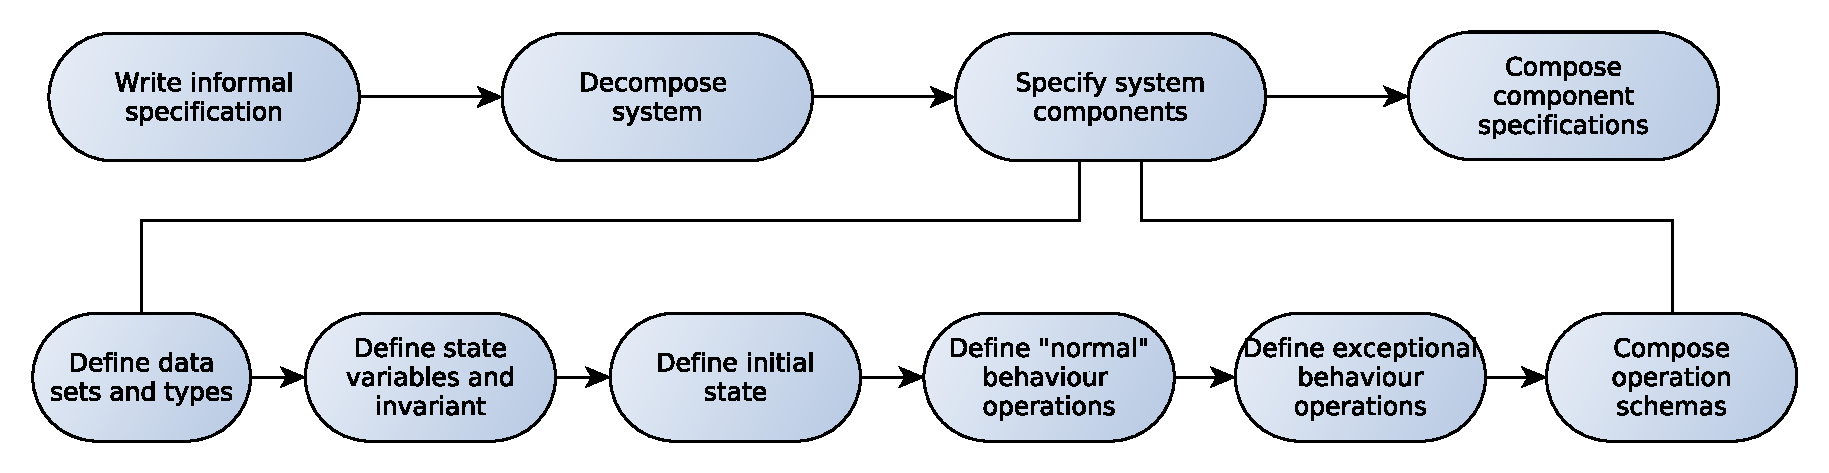
\includegraphics[scale=0.5]{\rootdir/specification/figures/specification-process}
\caption{A process to develop a model-based specification of a system.}
\label{fig:specification:specification-process}
\end{figure}

\subsubsection{State machines}

In these notes, we focus on the use of Alloy to specify and analyse abstract state machines: that is, an abstract model containing a \emph{state} (e.g.\ \A+PassBook+) and \emph{transitions} between these states. The LastPass password storage system defined in this chapter is one such example.

To do this, we used the \emph{abstract state machine} pattern. Using this pattern, we use predicates to specify operations on a global state. An abstract state machine in Alloy will have a structure something similar to:

\begin{alloy}
sig State { ... }
pred init [s: State] { ... }
pred inv [s: State] { ... }
pred op1 [s, s': State] { ... }
...
pred opN [s, s': State] { ... }
\end{alloy}

in which \A+init+ is the \emph{initialisation} operation, \A+inv+ is the \emph{state invariant}, and \A+Op1 ... OpN+ is a set of \emph{N} operations, such as \A+add+ and \A+delete+ in the password storage system. A state invariant is a formula that all operations in the specification must preserve.

\subsubsection{Operation preconditions}

We have already seen an example of splitting a precondition from its postcondition in an operation. However, an alternative way, which is preferred by many modellers, is to specify the precondition and postcondition together as separate predicates, and then bring them together in a single operation predicate. For example, we can declare operations \A+addPre+ and \A+addPost+ for the precondition and postcondition respectively, and then conjoin them in \A+addOk+:

\begin{alloy}
//True if and only if the user has no password for this URL
pred preAdd [pb: PassBook, url : URL, user: Username] {
    no pb.password[user][url] 
}

//Add a password for a user/url pair
pred postAdd [pb, pb': PassBook, url : URL, user: Username, pwd: Password] {
    pb'.password = pb.password + (user->url->pwd)
}

//Add a password for a *new* user/url pair
pred addOk [pb, pb': PassBook, url : URL, user: Username, pwd: Password] {
    preAdd [pb, url, user]
    postAdd [pb, pb', url, user, pwd] 
}
\end{alloy}

This has the effect of being more verbose, but providing a clear separation between the preconditions and the postconditions that specify the transitions, which many people find preferable.

\subsubsection{Exceptional cases}

An important step in Figure~\ref{fig:specification:specification-process} is the separation of ``normal'' cases from ``exceptional'' cases. The idea is to specify normal cases for a model first, which are usually the most difficult parts, and then to enumerate all the relatively-easier exceptional cases after this, many of which just ``fall into place''.

To achieve this, we specify the normal and exceptional cases in separate predicates, and then combine them using \emph{disjunction} in one operation predicate:

\alloyfile{linerange={43-65}}{\rootdir/specification/code/expanded_lastpass.als}

So, the \A+add+ predicate specifies an operation in which we attempt to add a duplicate entry, in which case nothing changes, \emph{or} the entry is not a duplicate, in which case we add the new entry.

Note the introduction of the variable \A+report : Report+, which is used as an output variable to specify whether the operation was successful or not. The \A+Report+ signature is declared as:

\alloyfile{linerange={23-26}}{\rootdir/specification/code/expanded_lastpass.als}

Thus, \A+report+ must take on a value from either \A+Success+ or \A+Failed+, which are disjoint sets.

This is useful in assertions where we can specify a case that we expect to e.g.\ fail, and check that it failed by simply checking that \A+report in Failed+.

\subsubsection{Invariant preservation}

When using the abstract state machine pattern, Alloy assertions provide the opportunity to check that the invariant is preserved by an operation, using the following template:

\begin{alloy}
assert initEstablishesInv {
  all s : State | init [s] => inv [v]
}

check initEstablishesInv

//for each operation
assert opNPreservesInv {
  all s : State, x : E, ... |
    inv [s] and opN [s, s', x : E, ... ] => inv [s']
}

check opNPreservesInv
\end{alloy}

This says that the initial state satisfies the state invariant, and for each operation, if the state invariant holds on state \A+s+, and we execute the operation, the state invariant holds on the post-state \A+s'+.

As an example, consider this for the \A+init+ and \A+add+ operations:

\alloyfile{linerange={99-106}}{\rootdir/specification/code/expanded_lastpass.als}

Such checks can be useful not only for checking state invariants, which may satisfy safety properties, but also to check sanity of operations.

For example, checking this assertion using the Alloy Analyser on the \A+delete+ operation actually revealed a fault that had not been detected before, which was subtle, but which modelled the semantics completely wrong. The line that removed the tuple from the \A+pb.passbook+ relation was:

\begin{alloy}
  pb'.password = pb'.password - (user->url->Password)
\end{alloy}

Can you see what the fault was?

This predicate states that \A+pb'.password+ is equal to \emph{itself} with the tuple subtracted. The second occurrence of \A+pb'+ should have been \A+pb+. This major semantic problem had not been discovered using check assertions  \A+deleteIsUndo+ and \A+deleteDuplicateDoesNothing+, due to a strange coincidence in how the operation was modelled and how the way these assertions were written.

\subsubsection{Summary}

So, by using the abstract state machine pattern, and structuring the model in a way that separates normal from exceptional behaviour, we can incrementally build up a model using a process such as the one in Figure~\ref{fig:specification:specification-process}.

Further, the abstract state machine pattern then lends itself naturally to some assertions such as checking whether invariants hold.

\section{Verification and validation}

As with any software engineering artefact, verification and validation (V\&V) are important. There are several techniques for V\&V of formal specifications:

\begin{enumerate}

 \item \emph{Animation}: Animation is the process of executing a specification with the intention of finding problems. The formal, unambiguous nature of specifications means that execution is often possible. However, because Alloy (and many other formal specification languages) is built on first-order logic, not all specifications are executable. 

 \item \emph{Model checking}: This is the process of attempting to execute every operation in every possible state of a system to show that certain properties hold; or more accurately, the find counterexamples of the properties. Model checking for model-based languages is difficult because the sheer number of states may be exponentially large, if not infinite. There is a lot of research around  the world looking at how to reduce the number of states for model checking while maintaining its soundness.

  If you have taken the subject \emph{Modelling Complex Software Systems}, you would used model checking to detect deadlock and to prove temporal logic properties of concurrency models.

 \item \emph{Review}: The specification can be subject to peer review, like any other document. This remains one of the most important and useful style of review for formal specification, despite advanced tools that can reason about them automatically.

 \item \emph{Proof}: Automated proof is the holy grail of formal specification. Proof is the most valuable of all techniques, because, unlike animation, model checking, reviews, and testing, if a property about a model can be proved, then we can say with strong conviction that it is true (although in reality, there is always the possibility that the proof itself is wrong!). 

\end{enumerate}

In this section, we discuss proof in more detail. This is not a major part of the subject, however, proof is an important motivation as to why practitioners adopt formal methods in software and systems engineering. Woodcock and Davies \cite{woodcock-using-z} present a far more thorough and valuable use of proof in specification. In this section, we discuss the implications of proof and present a trivial example.

\subsubsection*{The importance of proof}

If we have a specification of a system, then by reasoning about it using proof, we are likely to detect problems. If we have not started implementing the system, this provides us with an opportunity to find those problems before they become costly to fix. Further to this, the very process of constructing a proof can assist us in finding new requirements. That is, if we notice that we cannot prove a property about a system because some exceptional state has not been considered, we may need to add a requirement for this exceptional state. As Woodcock and Davies state: ``\emph{The practice of proof makes for better specifications}''.

There is a commonly-held opinion that proof is not possible on large-scale systems. Industrial application of formal specification and proof shows this opinion to be wrong. Proof can be applied to real systems running in real environments, and can provide cost savings too. There are situations where proof is not relevant or necessary, but to high integrity systems especially, there are situations where it is desirable and almost necessary. There may be some situations where a sketch of a proof is sufficient. The trick in apply proof is to know which proofs are worth attempting, which are worth sketching, and which are worth leaving.

It is worth referencing the following quote:

\begin{quote}
``\emph{Things like even software verification, this has been the Holy Grail of computer science for many decades but now in some very key areas, for example, driver verification we're building tools that can do actual proof about the software and how it works in order to guarantee the reliability}." --- Bill Gates, Chairman of Microsoft, speaking at WinHEC 2002 in Seattle, Washington, USA.
\end{quote}

\subsubsection*{What can be proved?}

Proof is used in some high integrity systems for cases in which the outcome of failure is catastrophic; e.g.\ resulting in death or complete mission failure. The types of properties that can be proved vary, however, some interesting properties that have been proved about formal models include:

\begin{itemize}

 \item Proofs that certain security protocols cannot be cracked. More importantly, there have been cases of security protocols where proofs have demonstrated that they \emph{can} be cracked.

 The \emph{Needham-Schroeder Public-Key Protocol} is a protocol intended to provide mutual authentication between two parties communicating over a network, proposed by Roger Needham and Michael Schroeder in 1978. It was considered to be a failproof way to establish identity between two communicators, however, it was not until Gavin Lowe applied formal proof to the protocol in 1995 that it was discovered that the protocol failed to prevent ``man-in-the-middle'' attacks.

 \item Proofs about safety properties. Many safety-critical systems need to ensure certain safety properties hold. For example, railway signalling systems need to ensure that, given an intersection of tracks, at no stage will overlapping tracks both have non-red signals. That is, only one train will be allowed on the intersection at any time. These properties are specified a temporal logic properties, and it can be shown that a formal specification preserves these properties.

 \item In many life-critical systems, formal proof is applied to minimise the risk of causing harm or death. In many systems employed on NASA space missions, proof is applied to demonstrate that certain cases cannot go wrong. In particular, NASA has been known to reject entire proposals for systems on aerospace systems or life-support systems for astronauts unless model checking or proof have been used to demonstrate mission-critical properties (mainly around safety).

\end{itemize}

\subsubsection*{What can't proof do?}

It is important not to say that if we ``prove'' our specification, then it is correct. When we do proofs about a formal specification, we are only proving that certain properties hold. We can say with some conviction that, if our proof can be discharged, then the property holds. However, this is only valuable if the property is correct. Further, we can do many proofs on a system, but omit an important one. Thus, a set of proofs is only as strong as the set of properties they show.

In most cases, proofs are not automated. That is, we cannot provide a specification and a property, and then have it proved. There are a large set of proofs for which this is possible, but there is another set for which it is currently not. The holy grail of theorem proving is exactly to prove things automatically, but for now, it remains a pipedream. For many logics, it has been proved that not all provable properties of the system can be automatically proved.

\subsubsection*{An example}

As a small example of how proof words, we'll use the chemical storage system outlined in Chapter~\ref{chapter:safety}.

\begin{example}

In the chemical storage system, the storage tank has a maximum limit, and if that limit is breached, serious safety consequences may result.
However, the overfilling problem is resolved using careful specification, and we can prove that the storage tank will not overflow, providing our specification is implemented correctly.

If we consider a \texttt{Fill} operation for filling the take, it will consist of a precondition checking that the amount going into the tank will not overflow, and a postcondition calculating the new amount. The safety property we want to check is that the new amount does not overlow the tank:

\begin{itemize}

 \item \emph{Precondition}: $contents + amount? \leq capacity$

 \item \emph{Postcondition}: $contents' = amount? + contents$

 \item \emph{Safety property}: $contents' \leq capacity$ (which is also the state invariant).

\end{itemize}

We can then structure our proof as follows:

\begin{center}
$Precondition \implies (Postcondition \implies Safety\ property)$
\end{center}

That is, if the precondition is true, then the postcondition implies that the safety property holds.

For the \texttt{Fill} operation, this is straightforward to discharge. We have to prove:

\quad  $contents + amount? \leq capacity ~\implies$

\vspace{-2mm}

\quad\quad $(contents' = contents + amount? \implies contents' \leq capacity)$

Using the \emph{one-point rule}, we can replace all instances of \texttt{contents'} with \texttt{contents + amount?}: 

\quad  $contents + amount? \leq capacity \implies~$

\vspace{-2mm}

\quad\quad $(contents + amount? = contents + amount? \implies contents + amount? \leq capacity)$

The middle proposition $contents + amount? = contents + amount?$ is trivially true, so can be removed from the entire proposition, leaving:

\quad  $contents + amount? \leq capacity \implies contents + amount? \leq capacity $,

which is itself trivially true.

So, we have \emph{proved} that, for every possible state of the system, if the precondition holds, the storage container will not be filled beyond capacity. This is much stronger than throwing a million tests at it to see if we can find an input/state pair that violates it.

\end{example}

The above example is trivial in comparison to the types of proofs that are discharged on industrial scale systems, however, it illustrates how proof can be applied to a model-based specification.

Despite the small size, the proof required a few steps are several lines of text.  However, significant tool support is available for theorem proving. Using automated and interactive theorem provers, many large proofs can be discharged in a fairly straightforward manner, and the documentation of the proof can be generated automatically and stored digitally.


% LocalWords:  lifecycle Abrial Sommerville VDM statecharts PDF LMS
% LocalWords:  schemas nat powerset GivenType aboveskip sc FreeType
% LocalWords:  ModuleName dec pred linerange OperationName pre init
% LocalWords:  postconditions PrimaryColours forall emptyset structs
% LocalWords:  LargeSchema LeftSchema RightSchema PostFill GSM EF DF
% LocalWords:  EFs DFs mf df gsm ef dl dr iccid ddl ddr acm nia imsi
% LocalWords:  PINs PUK PUKs ALW CHV CICS el issubset GSMFiles chv lp
% LocalWords:  GSMSecurity SchemaName WinHEC Needham failproof FillOK
% LocalWords:  OverFill NewVariable OldVariable pipedream logics lll
% LocalWords:  FillTwice implementers disjunction satisifiability ur
% LocalWords:  usernames LastPass username unary myUsername tuples pb
% LocalWords:  myPassword urlPasswords rddd uur myUrl newPassword iff
% LocalWords:  someUsernames somePasswords tuple myUserName pwd sig
% LocalWords:  myUserame Cardinalities PassBook url PassBoook preAdd
% LocalWords:  invariants renamings lookup satisfiable unsatisfiable
% LocalWords:  addWorks infeasible inv opN addPre addPost addOk
% LocalWords:  initEstablishesInv opNPreservesInv deleteIsUndo
% LocalWords:  deleteDuplicateDoesNothing provers
